% !TEX TS-program = xelatex
% !TEX encoding = UTF-8

% This is a simple template for a XeLaTeX document using the "article" class,
% with the fontspec package to easily select fonts.

\documentclass{book} % use larger type; default would be 10pt

\usepackage{pdfpages}
\usepackage{tcolorbox}
\usepackage{tabularx}
\usepackage[margin=1in]{geometry}
\usepackage{algorithm}
\usepackage{algorithmic}
\usepackage{xepersian}

\settextfont{Yas}
\setlatintextfont{Bitstream Charter}
\setdigitfont{Yas}


\renewcommand{\labelitemi}{$\bullet$} % fix persian items

\newcommand{\imgcaption}[1]{\color[HTML]{4F4D4D}\footnotesize{#1}}

\linespread{1.5}

\begin{document}


\title{طراحی الگوریتم: پیشرفتهای روشمند}
\author{حسین رادمرد}
\date{15 اردیبهشت 1403}
%\date{} % Activate to display a given date or no date (if empty),
         % otherwise the current date is printed 

\maketitle

\section{مسئله 83 رنگ کردن یک گراف دو رنگی}

در این مسئله، مانند موارد بعدی، حل مسئله هدف ماست و بهینه بودن جواب برای ما حائز اهمیت نیست. دراینجا، ما الگوریتمی را برای رنگ کردن گراف با دردست داشتن تنها دو رنگ، بررسی میکنیم. نسخه‌ی کلی‌تر(رنگ آمیزی با هر تعداد رنگ) در مسئله‌ی 59، صفحه‌ی 236 بررسی میشود. گرچه، نسخه‌ی فعلی بسیار بهینه‌تر است. در ادامه، این بحث بسیار به موضوع "گرافهای پرکاربرد: گراف‌های دوبخشی" مرتبط است.

گراف همبند بدون جهت 
${(G = N, V)}$
 (ناتهی) به ما داده شده‌ست. ما قصد داریم با رنگ‌های سیاه و سفید گراف را رنگ آمیزی کنیم به گونه‌ای که هیچ دو راس همسایه‌ای دارای رنگ یکسانی نباشند. چنین گرافی را گراف دورنگی مینامیم. الگوریتم حریصانه ای که ما قصد ساخت آن را برای این منظور داریم به پیمایش سطری گراف ها مرتبط است که آن را در ابتدا بررسی کردیم.


 چنین گرافی را گراف دورنگی مینامیم. الگوریتم حریصانه ای که ما قصد ساخت آن را برای این منظور داریم به پیمایش سطری گراف ها مرتبط است که آن را در ابتدا بررسی کردیم.
\subsection*{پیمایش سطری گراف: یادآوری}
\subsubsection*{معرفی}

اول از همه، اجازه دهید مفاهیم "فاصله‌ی میان دو راس" و "پیمایش سطری" را برای گراف‌های همبندِ بدون جهت تعریف کنیم.

تعریف 10 (فاصله‌ی میان دو راس):
در نظر میگیریم، $G = (N, V)$ یک گراف همبند بدون جهت و s و s' دو راس این گراف باشند. طول کوتاه‌ترین مسیر میان s و s' را فاصله‌ی میان s و s' گویند.


تعریف 11 (جستجوی سطری):
فرض کنیم G یک گراف همبند و بدون جهت و s یکی از راس های آن باشد. هر فرایندی که با افزایش فاصله‌ها از راس s با راس های گراف G برخورد میکند به عنوان پیمایش سطری گراف G از s شناخته میشود.  



از نمودار (b) در شکل 7.8 صفحه‌ی 363، میتوانیم نتیجه بگیریم که لیست $⟨a, b, c, d, e, f, g, h⟩$ با پیمایش سطری با شروع از راس a مطابقت دارد. و همین مطلب برای لیست $⟨a, c, b, d, e, h, f, g⟩$ نیز صدق میکند.


\begin{center}
    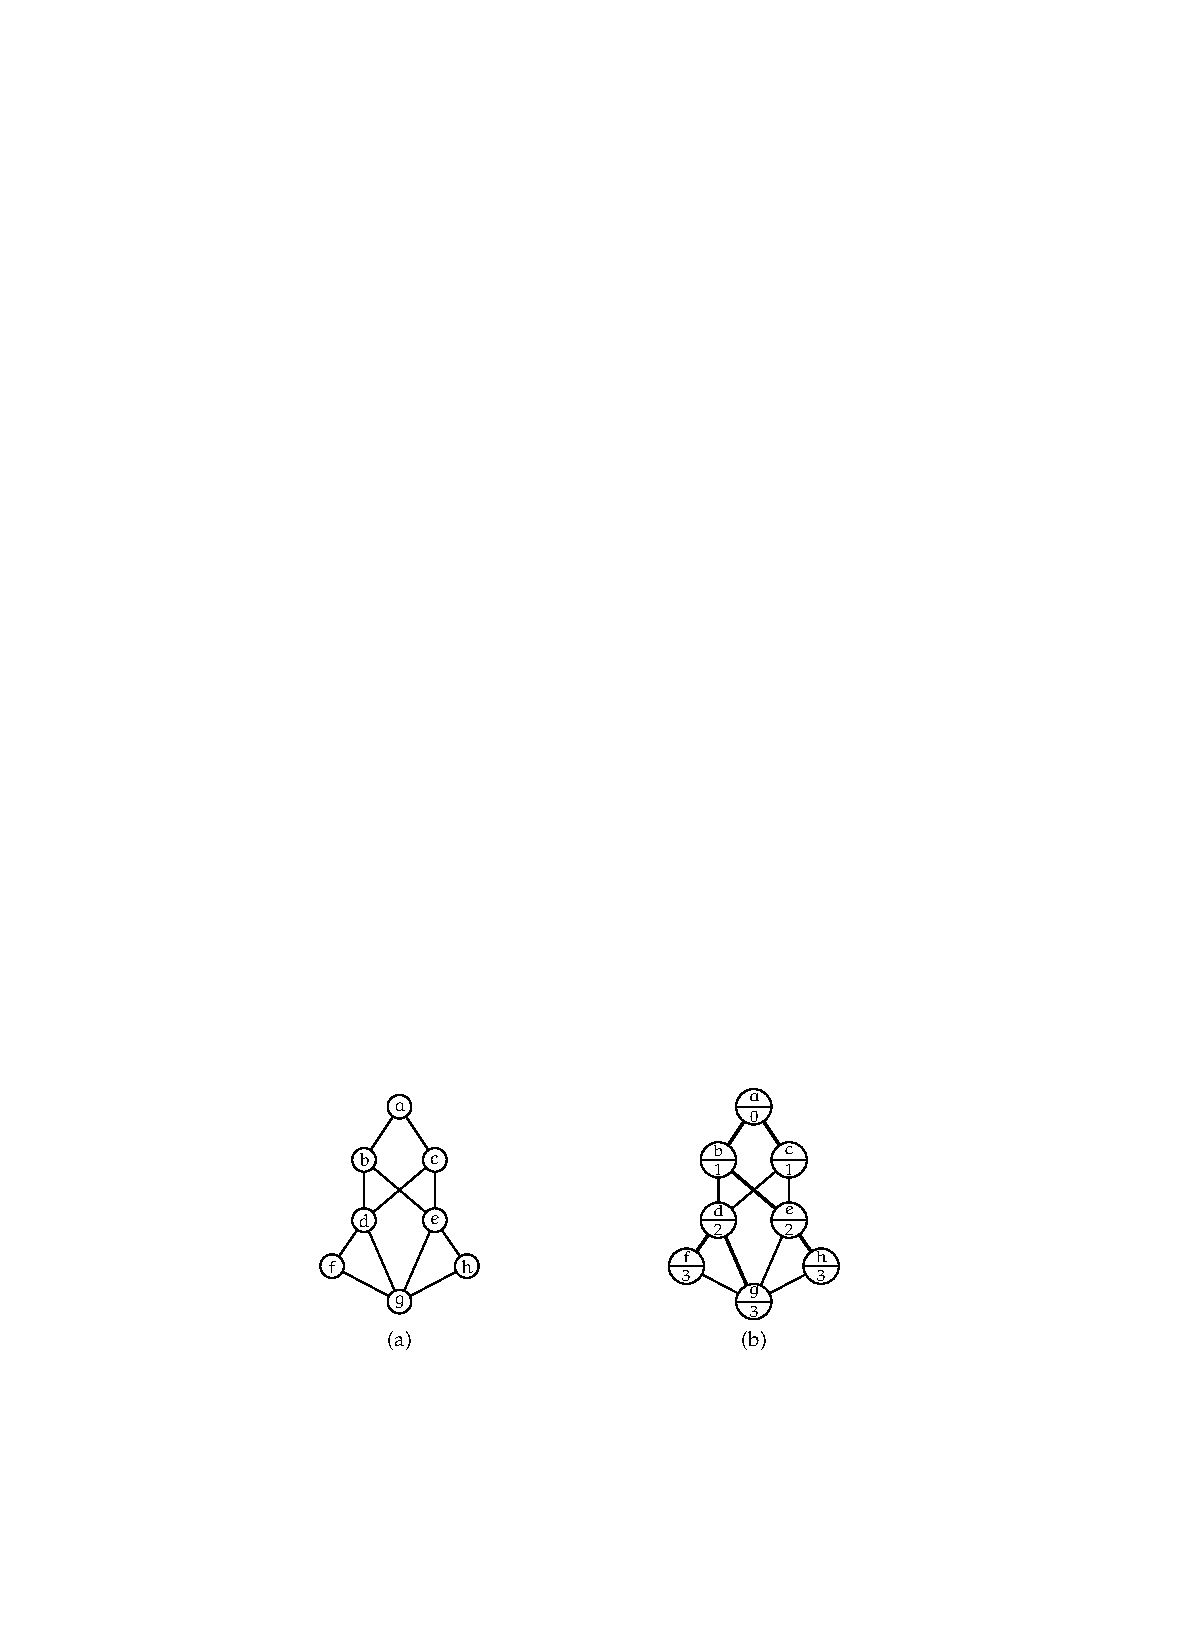
\includegraphics{./fig7.8.pdf}

    % \imgcaption{جدول ۱۲.۱۲: یک آرایه پیشوند-پسوندی از تمام پورین های ۴ حرف}
\end{center}

تصویر 7.8 - یک مثال از گراف. تصویر (a) گرافی را نمایش میدهد که مثالی از حالت مسئله را نشان میدهد.  تصویر (b) کوتاه‌ترین مسیر راس a را تا هر راس گراف با خطوط پررنگ نشان میدهد. در تصویر (b)، عددی که در هر راس مشخص است در واقع فاصله‌ی آن راس تا راس a است.



%\subsection{}
\newpage
\subsubsection*{حلقه بدون تغییر}

ما علاقه داریم یک الگوریتم حریصانه تکرارشونده بسازیم، و در این نمونه خود را برای جستجوی حلقه بدون تغییر محدود میکنیم، ادامه ی این ساز و کار به خواننده واگذار میشود. اکنون تصور میکنیم قسمتی از کار انجام شده ست(بخش ۳، صفحه ۹۳ را ببنید). به این ترتیب، برای یک گراف جزئی $G′ = (N′, V′)$ (زیرگراف G القا شده با مجموعه رئوس $N'$، حاوی راس شروع s)، لیستی تشکیل شده از پیمایش سطری $G'$ با شروع از s داریم.
مرسوما، این لیست، CLOSE نامیده میشود. پیشرفت این روند شامل گستردن این لیست با افزودن رئوسی است که در CLOSE نیستند و تا جای ممکن به s نزدیکند.


از آنجایی که هر راسی که در CLOSE حضور نداشته باشد، یک کاندید احتمالی برای انقال به CLOSE است، در غیاب بقیه ی مفروضات، پیشرفت ممکن اما به همان نسبت هزینه بر است.
پیشنهاد میکنیم که نسخه اول این ثابت را با اضافه کردن یک ساختمان داده بهبود ببخشید. ساختمان داده OPEN شامل تمام رئوسی ست که در CLOSE حضور نداشته و کاندید این موضوع هستند که همسایه حداقل یکی از رئوس CLOSE هستند.
بیشین\LTRfootnote{priori}، OPEN به عنوان یک لیست اولویت با مدیریت برروی فاصله ی عناصرش از ‌s بوجود می آید، این موضوع به این دلیل است که عنصری که باید به لیست CLOSE منتقل شود باید نزدیک ترین به s باشد.


بعدها میبینیم که نسخه ساده تری از یک لیست اولویت نیز امکان پذیر است. برای ماندگاری این نسخه جدید از تغییرناپذیر \LTRfootnote{invariant}، بهینه است که ابتدای صف OPEN را به انتهای لیست CLOSE، - به عنوان همتای تقویت ثابت** - برای معرفی همسایگان "جدید" عنصر منتقل شده به OPEN، عنصرهایی که نه در OPEN نه در CLOSE هستند(انتخاب حریصانه) منتقل کنیم.

با این حال، با توجه به عنصر e در OPEN، پرسیدن سوال درباره وجود یا عدم وجود یکی از همسایگان آن در OPEN یا CLOSE می تواند پرهزینه باشد. راه حل بهتر شامل گزاره زیر است: از نظر رنگ آمیزی، یک "رنگ" به هر راس گراف اختصاص می یابد؛ سفید، اگر راس در OPEN یا CLOSE باشد، و در غیر این صورت خاکستری (در واقع، در اینجا، دو رنگ نقش مقادیر بولین را بازی می کنند). به شرطی که دسترسی مستقیم به رئوس امکان پذیر باشد، به روز رسانی OPEN آسان تر می شود. در پیشرفت، حفظ این مکمل نامتغییرا با رنگ آمیزی هر راسی که به OPEN منتقل می شود به رنگ سفید حاصل می شود.

بیایید به استراتژی مدیریت صف OPEN بازگردیم. آیا می توان به جای صف اولویت دار از یک صف ساده FIFO (نگاه کنید به بخش 1.8، صفحه 32) استفاده کرد؟ در این صورت، مدیریت OPEN به طور قابل توجهی ساده می شود. برای انجام این کار، زمانی که رأس e از OPEN خارج می شود تا به CLOSE ملحق شود، همسایگان e که نامزد ورود به OPEN هستند باید فاصله ای بیشتر یا مساوی با تمام عناصر موجود در OPEN داشته باشند، که این امر امکان داشتن یک صف مرتب را فراهم می کند. این بدان معناست که اگر e در فاصله k از s باشد، سایر عناصر OPEN در فاصله k یا $(k + 1)$ از s قرار دارند، زیرا همسایگان "خاکستری" e در فاصله $(k + 1)$ از s قرار دارند. این فرض را به نامتغییرا اضافه می کنیم. خواننده دعوت می شود بررسی کند که آیا این موضوع با راه‌اندازی حلقه واقعاً برقرار شده است. همچنان باید ثابت کرد که با پیشرفت حفظ می شود. در نهایت، ما نامتغییرای زیر را پیشنهاد می کنیم که از چهار بند تشکیل شده است.

\begin{enumerate}
    \item  بسته (CLOSE) یک صف اول-وارد-اول-خارج (FIFO) است که محتوای آن نشان دهنده یک "پیمایش عمق-اول" از زیرگراف G است که توسط رئوس موجود در بسته (CLOSE) تشکیل شده است.
    
    \item  باز (OPEN) یک صف اول-وارد-اول-خارج (FIFO) از رئوس همسایه رئوس موجود در بسته (CLOSE) است. اشتراک مجموعه بین باز (OPEN) و بسته (CLOSE) تهی است.

    \item اگر ابتدای صف باز (OPEN) حاوی رئوس با فاصله k از s باشد، سایر عناصر صف باز (OPEN) در فاصله k یا $(k + 1)$ از s قرار دارند.

    \item در گراف G، رئوس موجود در بسته (CLOSE) یا باز (OPEN) به رنگ سفید رنگ آمیزی می شوند، سایر رئوس خاکستری هستند.
\end{enumerate}
\newpage

شکل ۷.۹، صفحه ۳۶۶، مراحل مختلف «پیمایش اول-سطر» گراف شکل ۷.۸، صفحه ۳۶۳ را نشان می‌دهد. در هر گراف موجود در تصویر، رئوس موجود در CLOSE با خطوط خاکستری و رئوس موجود در OPEN با خطوط دوتایی نمایش داده شده‌اند. فواصل فقط به عنوان یادآوری ذکر شده‌اند، الگوریتم از آنها استفاده نمی‌کند. بیایید به عنوان مثال در مورد مرحله‌ای که منجر به گذار از شکل e به شکل f می‌شود، توضیح دهیم. در شکل e، لیست CLOSE «پیمایش اول-سطر» زیرگراف القا شده توسط رئوس a، b، c و d را در خود جای داده است. راس e، ابتدای صف OPEN، به انتهای CLOSE منتقل خواهد شد. کدام همسایه‌های e قرار است به OPEN ملحق شوند؟ c و b از قبل در CLOSE هستند، بنابراین آنها را در نظر نمی‌گیریم. g از قبل در OPEN است، بنابراین تحت تأثیر قرار نمی‌گیرد. تنها راس باقی‌مانده h است که به صف OPEN ملحق شده و با رنگ سفید رنگ‌آمیزی می‌شود.

\subsubsection*{ساختارهای داده}

از دو نوع ساختار داده در این الگوریتم استفاده شده است. مورد اول، صف‌های اول-وارد-اول-خارج\LTRfootnote{FIFO: first in first out}، که در صفحه ۳۲ توضیح داده شده‌اند. مورد دوم مربوط به نسخه‌ی «رنگ‌آمیزی‌شده» گراف‌ها است.
این ساختار داده را گراف بدون جهت رنگ‌آمیزی‌شده می‌نامند.

در این الگوریتم، نیاز به رنگ‌آمیزی رئوس‌های یک گراف، دسترسی به رنگ آن‌ها و کاوش لیست همسایگان وجود دارد، بنابراین تعاریف زیر ارائه می‌شود (فرض بر این است که مجموعه رنگ‌ها تعریف شده است):


\begin{itemize}
    \item عملگر رنگ‌آمیزی‌ $ColorGr(G, s, col)$: عملیاتی که رأس s گراف G را با رنگ col رنگ‌آمیزی می‌کند.
   
    \item عملگر $ColorGr(G, s, col)$: عملیاتی که رأس s گراف G را با رنگ col رنگ‌آمیزی می‌کند.
    \item تابع $WhichColorGr(G, s)$ نتیجه رنگ‌ها: تابعی که رنگ رأس s گراف G را برمی‌گرداند.
    \item عملگر $OpenNeighborsGr(G, s)$: عملیاتی که کاوش لیست همسایگان رأس s گراف G را آغاز می‌کند.
    \item تابع $EndListNeighborsGr(G, s)$ نتیجه بولی: تابعی که مقدار درست را برمی‌گرداند اگر و تنها اگر کاوش لیست همسایگان رأس s گراف G تمام شده باشد.
    \item عملگر $ReadNeighborsGr(G, s, s′)$: عملیاتی که هویت رأسی که زیر نشانگر لیست همسایگان s است را در s′ ذخیره کرده و سپس نشانگر را یک خانه به جلو حرکت می‌دهد.
    
\end{itemize}

در این کاربرد، از نظر بیان الگوریتم و کارایی، بهترین بهینه‌سازی نمایش آن با استفاده از لیست همسایگی است (برای مشاهده‌ی نمونه‌ای از چنین نمایشی برای گراف‌های جهت‌دار، به شکل d در صفحه‌ی ۲۳ مراجعه کنید). بنابراین، گراف به صورت یک "سه‌تایی" $G = (N, V, R)$ تعریف می‌شود که در آن R نشان‌دهنده رنگ‌ها است (در حال حاضر "سفید" و "خاکستری").

\subsubsection*{الگوریتم}

علاوه بر نمودار G، این الگوریتم از متغیرهای cv راس جاری و فهرست همسایگان برای مرور لیست همسایگان استفاده می کند.


\begin{latin}
    
    \begin{algorithm}
        % \caption{}\label{your_label}
        \begin{algorithmic}
            \STATE $constants:$
            \STATE n $\in$ N1 and n = . . . and N = 1 .. n and Colors = {grey, white} and
            \STATE V $\in$ N × N and V = {. . .}
            \STATE $variables:$
            \STATE R $\in$ N → Colors and G = (N, V, R) and
            \STATE s $\in$ N an d cv $\in$ N and neighb $\in$ N and CLOSE $\in$ FIFO(N) and OPEN $\in$ FIFO(N)
            \STATE $begin$
        \end{algorithmic}
    \end{algorithm}
        
\end{latin}

\begin{center}
    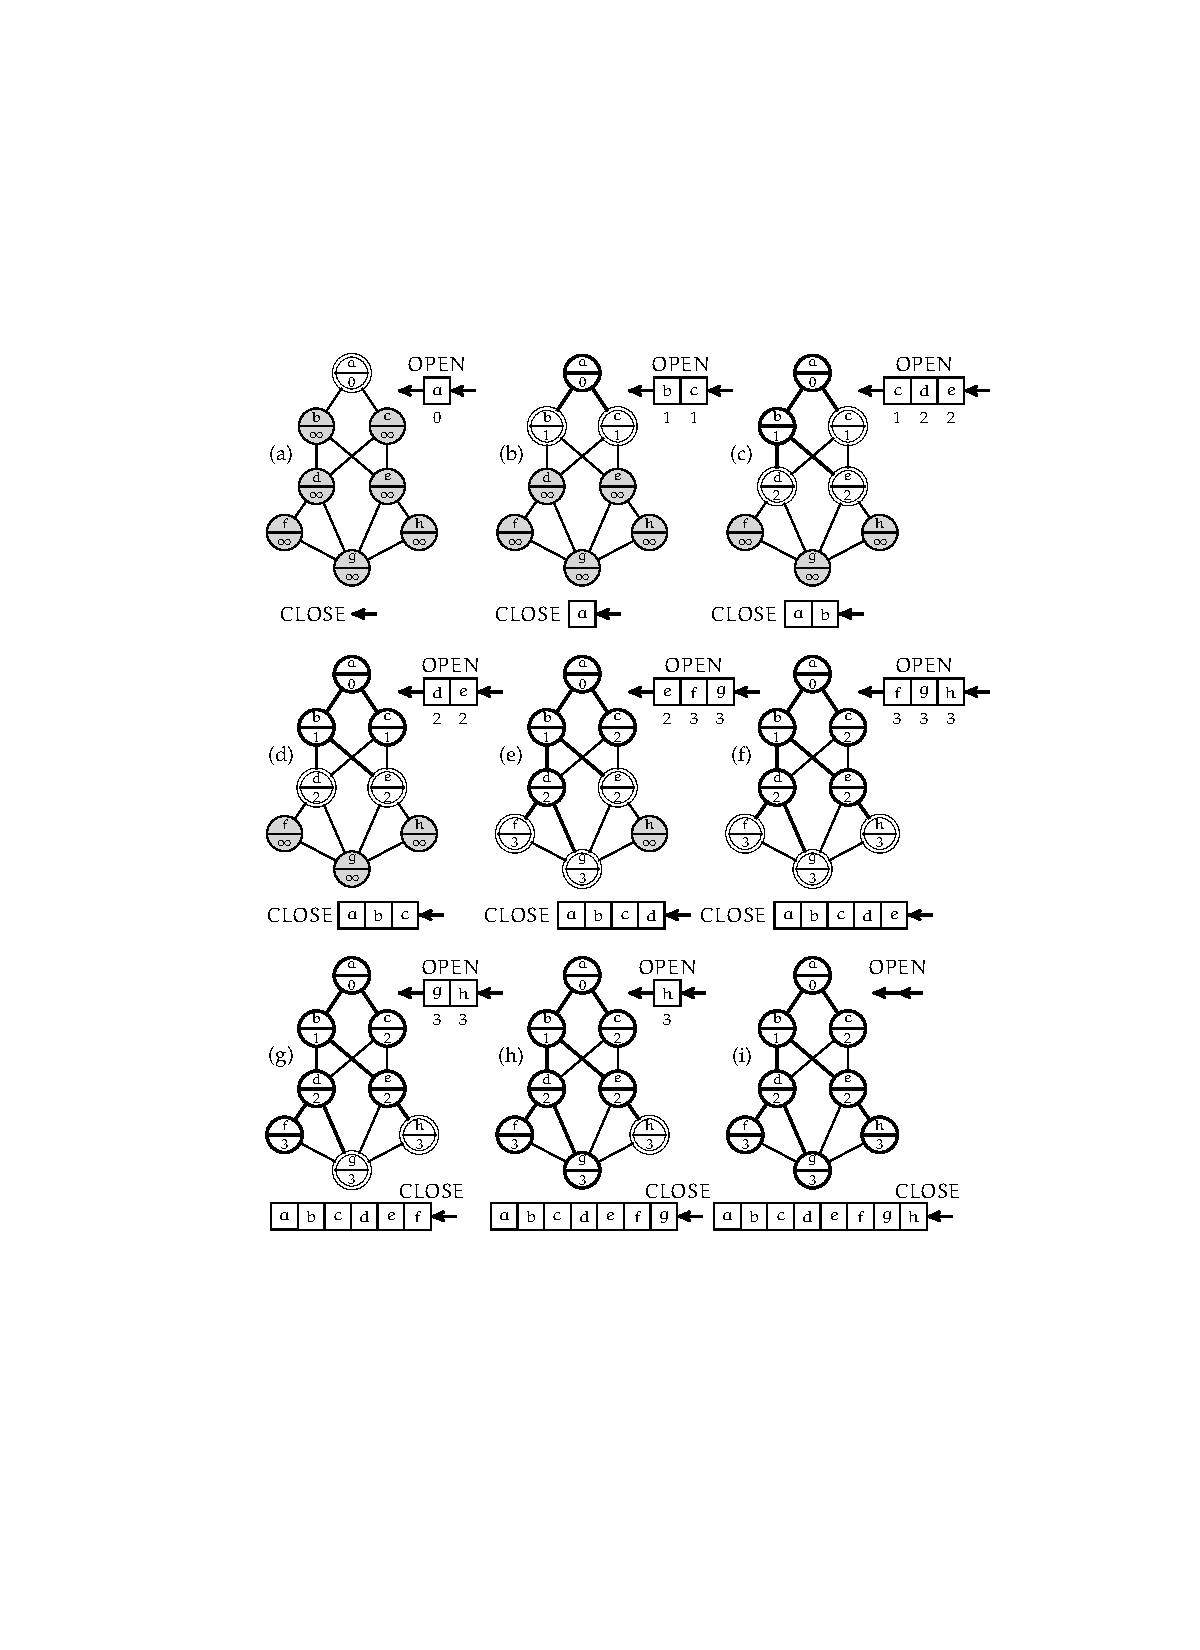
\includegraphics{./fig7.9.pdf}

    % \imgcaption{جدول ۱۲.۱۲: یک آرایه پیشوند-پسوندی از تمام پورین های ۴ حرف}
\end{center}

شکل 7.9 - مراحل مختلف کاوش اولویت-عرضی در گراف اسکیما (الف) در شکل 7.8 (صفحه 363). رئوس با دایره توپر، رئوس CLOSE هستند، آنهایی که با دو دایره مشخص شده اند، رئوس OPEN هستند. مقدار صحیح که هر راس را همراهی می کند، فاصله شناخته شده از راس a است. دو صف OPEN و CLOSE به ترتیب در شمال شرقی و جنوب گراف ها نشان داده شده اند.

\begin{latin}
    
    \begin{algorithm}
        \caption{}\label{your_label}
        \begin{algorithmic}
            \STATE //coloring all the vertices in grey:
            \FOR{$w \in N$}
                \STATE $ColorGr(G, w, grey)$
            \ENDFOR
            \STATE $InitFifo(CLOSE); InitFifo(OPEN);$
            \STATE $s \leftarrow$ . . . ; // choice of the initial vertex:
            \STATE $ColorGr(G, s, white);$
            \STATE $AddFifo(OPEN, s);$
            \WHILE{not $IsEmptyFifo(OPEN)$}
                \STATE $cv \leftarrow HeadFifo(OPEN); RemoveFifo(OPEN);$
                \STATE $AddFifo(CLOSE, cv);$
                \STATE $OpenNeighborsGr(G, cv);$
                \WHILE{not $EndListNeighborsGr(G, cv)$}
                    \STATE $ReadNeighborsGr(G, cv, neighb);$
                    \IF{$WhichColorGr(G, neighb) = grey$}
                        \STATE $ColorGr(G, neighb, white);$
                        \STATE $AddFifo(OPEN, neighb);$
                    \ENDIF
                \ENDWHILE
            \ENDWHILE
            \STATE $write(CLOSE);$
            \STATE $END$
        \end{algorithmic}
    \end{algorithm}
        
\end{latin}

سوال ۱: پیچیدگی مجانبی این الگوریتم از نظر شرایط ارزیابی شده چیست؟

سوال ۲: بر اساس این الگوریتم، اصل الگوریتم رنگ آمیزی حریصانه را توضیح دهید.

\subsection*{الگوریتم رنگ آمیزی دو رنگ گراف}

اکنون تمام چیزی که برای حل مسئله نیاز است را داریم تا به مشکل اصلی در هسته این مسئله بپردازیم: رنگ آمیزی یک گراف با سیاه و سفید. ما الگوریتم بالا را به گونه ای تطبیق خواهیم داد که به صورت متناوب با سیاه و سفید، بر اساس عمق در رابطه با راس شروع، رنگ آمیزی شود، تا زمانی که رئوس تمام شوند یا به یک حالت غیرممکن برخورد کنیم.

سوال ۳: الگوریتم رنگ آمیزی را طراحی کنید.

سوال ۴: بر اساس این الگوریتم، اصل الگوریتم رنگ آمیزی حریصانه را توضیح دهید.

شکل ۷.۸، صفحه ۳۶۳

سوال ۵: کد الگوریتم را بنویسید و پیچیدگی آن را مشخص کنید.

سوال ۶: مسئله 59، صفحه 236، به مسئله عمومی‌تر رنگ‌آمیزی با m رنگ $(m \geq 2)$ می‌پردازد.
امکان تعمیم الگوریتم ارائه شده در پاسخ به سوال 5، برای m > 2 را مورد بحث قرار دهید.

تذکر
یک ویژگی جالب از گراف‌های دو-رنگ‌پذیر این است که: یک گراف، دو-رنگ‌پذیر است اگر و تنها اگر هیچ دوری با طول فرد نداشته باشد. با این حال، این ویژگی سازنده نیست: مشاهده‌ی آن روی یک گراف منجر به رنگ‌آمیزی نمی‌شود!

راه‌حل در صفحه ۳۹۷ است.

\newpage

\subsection {مسئله ۸۴: از ترتیب جزئی به ترتیب کلی}

دو نسخه از مرتب‌سازی توپولوژیکی مورد بررسی قرار می‌گیرد. نسخه اول ساده لوحانه است
اما خیلی کارآمد نیست و طراحی آن آسان است. نسخه دوم نیازمند تقویت یک نامتغیر است؛ با استفاده از اشاره‌گرها پیاده‌سازی می‌شود و هر دو مسئله‌ی بهینه‌سازی و
استفاده از ساختارهای پویا را به خوبی نشان می‌دهد. الگوریتمی که در اینجا ساخته شده است
نزدیک به الگوریتم ماریمونت برای سطح‌بندی یک گراف بدون مدار است.

برای حل این مسئله، ابتدا باید مسئله ۲، صفحه ۳۳ را بررسی کرد.
فرض کنید $(E, \prec)$ یک زوج مرتب باشد به گونه‌ای که E یک مجموعه متناهی با n عضو
و $\prec$ یک رابطه ترتیب جزئی روی E باشد. ما می‌خواهیم روی E یک رابطه ترتیب کلی
$\le$ سازگار با $\prec$ بنا کنیم، به این معنی که برای هر زوج $(a, b)$ از $E: (a \prec b) \rightarrow (a \le b)$.
به هر عضو از $(E, \prec)$ که هیچ پیش‌تر نداشته باشد، عضو مینیمال گفته می‌شود.


مثال
در زمینه‌ی دوره‌ی علوم کامپیوتر، $c1 \prec c2$ نشان‌دهنده‌ی این موضوع است که دوره‌ی c1 باید
قبل از دوره‌ی c2 گذرانده شود تا پیش‌نیازهای لازم برای درک دوره‌ی دوم فراهم شود.
حال دوره‌های زیر را در نظر بگیرید:


% \begin{table}[]
%     \begin{tabular}{lllll}
%     a & منطق مرتبه اول  & b & مشخصات و برنامه نویسی ضروری & \\
%     c & نظریه مجموعه    & d & طراحی سیستم های اطلاعاتی    & \\
%     e & پایگاه های داده & f & داده ساختارها               & \\
%     \end{tabular}
% \end{table}

\begin{tabularx}{0.8\textwidth} { 
    | >{\arraybackslash\arraybackslash}X 
    | >{\centering\arraybackslash}X 
    | >{\raggedleft\arraybackslash}X 
    | >{\raggedleft\arraybackslash}X
    | >{\raggedleft\arraybackslash}X |}
   \hline
   a & منطق مرتبه اول & b & مشخصات و برنامه نویسی ضروری \\
   \hline
   c & نظریه مجموعه & d &  طراحی سیستم های اطلاعاتی \\
  \hline
   e & پایگاه های داده & f & داده ساختارها \\
  \hline
\end{tabularx}


مثالی از رابطه $\prec$ به صورت زیر تعریف می‌شود:

$a \prec b, a \prec c, b \prec d, c \prec b, c \prec d, c \prec e, c \prec f, e \prec d, f \prec e$.

این را می‌توان با نمودار زیر نشان داد:

\begin{center}
    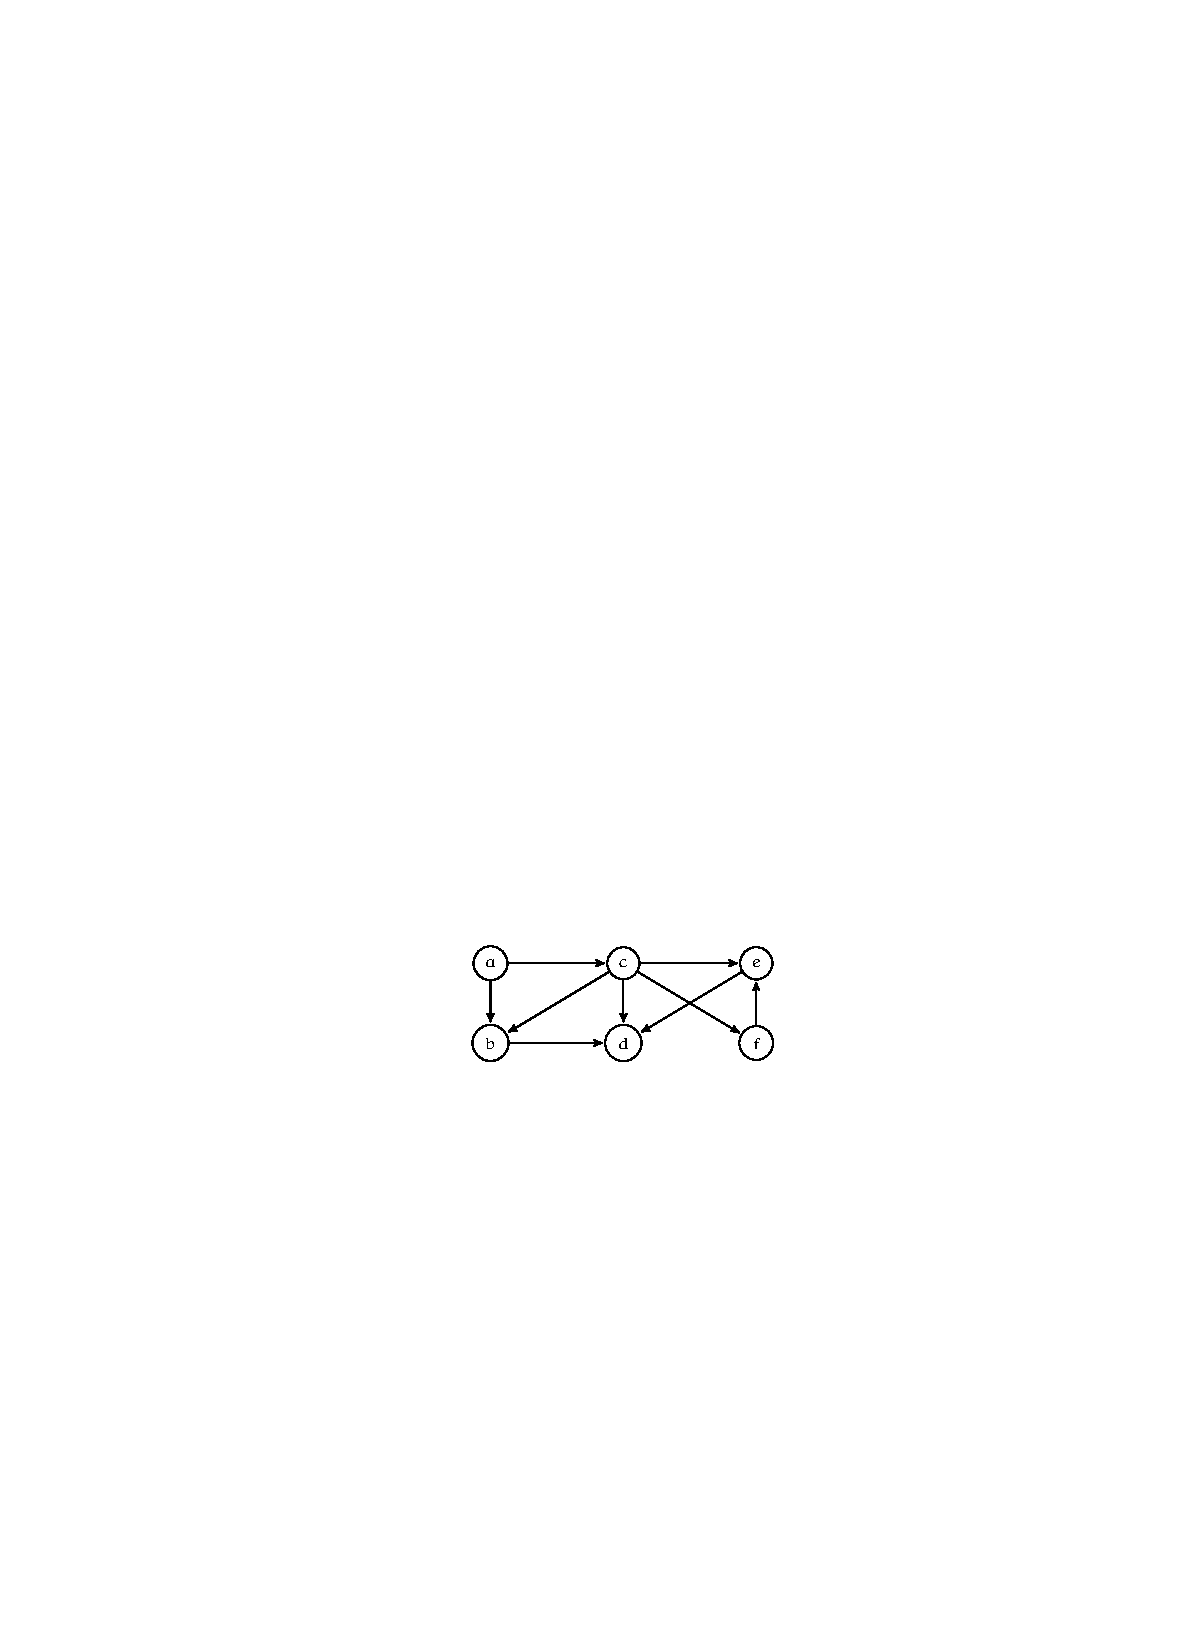
\includegraphics{./fig7.10.pdf}

    % \imgcaption{جدول ۱۲.۱۲: یک آرایه پیشوند-پسوندی از تمام پورین های ۴ حرف}
\end{center}

این نوع گراف با دو ویژگی شناخته می‌شود: جهت‌دار بودن و عاری بودن از دور. به چنین گرافی، «گراف جهت‌دار بدون دور» یا «DAG» گفته می‌شود. در چنین
گرافی به یک عضو بدون هیچ پیش‌تر \LTRfootnote{predecessor} (عضو مینیمال مرتب‌سازی جزئی)، «نقطه‌ی ورود»
گفته می‌شود.

هدف این مسئله، ساخت یک الگوریتم حریصانه است که یک ترتیب کلی سازگار با ترتیب جزئی اولیه را ارائه دهد. برای مثال بالا، یک راه‌حل شامل پیشنهاد ترتیب کلی $a \le c \le b \le f \le e \le d$ است.

سوال 1: اثبات کنید که یک گراف جهت‌دار غیر دوردار (DAG) غیر تهی، که هر یک از نقاط ورود آن حذف
شده باشد، همچنان یک گراف جهت‌دار غیر دوردار (DAG) باقی می‌ماند.


سوال 2: فرض کنیم هر گرافی با $G = (N, V)$ نمایش داده شود و n برابر $card(N)$ باشد.
اثبات کنید که برخی DAG ها (گراف جهت‌دار بدون دور) به گونه‌ای هستند که $card(V) \in \Theta (n^2)$
است.

اکنون، پیش از اجرای آن روی مثال بالا، به ترسیم کلی حلقه‌ی “حریصانه” الگوریتم می‌پردازیم.
روش ساخت استفاده شده مبتنی بر تکنیکِ «اجرای پیشرو» است. سوالات بعدی در مورد
الگوریتم، بهینه‌سازی و پیچیدگی آن خواهد بود.

\newpage

\subsubsection*{اولین تلاش برای ساخت}
فرض کنید $G = (E, V)$ یک DAG ورودی با n راس باشد

نامتغییر: فرض کنید S صف خروجی باشد که شامل مجموعه $E_{S} (E_{S} \subseteq E)$ از رأس‌های مرتب‌سازی‌شده بر اساس یک ترتیب کلی سازگار با $\prec$ می‌باشد، به گونه‌ای که هر راس v از $E$ که در $E_{S}$ نیست $(v \in (E - E_{S} ))$ طبق ترتیب جزئی بزرگ‌تر از هر راس $E_{S}$ است.

شرط توقف: تمام رأس‌ها در صف S قرار دارند، یعنی $|S| = n$.
در واقع، اشتراک نامتغییر و شرط قبلی ایجاب می‌کند که S
فهرستی مرتب‌سازی‌شده بر اساس ترتیبی سازگار با ترتیب جزئی باشد.

روند کار الحاق یکی از رأس‌های $(E - E_{S} )$ به صف S است.
این کار باعث می‌شود که این راس در زیرگراف القا شده $(Induced(G, E - E_{S} ))$ قرار گیرد
و نامتغییر در این راستا تقویت خواهد شد.

به منظور تعیین راسی که باید به بهترین نحو در صف قرار گیرد، ضروری است یک ساختار
داده‌ای معرفی کنیم که قادر به بهره‌برداری از زیرگراف القا شده $(Induced(G, E - E_{S} ))$ باشد.

\subsubsection*{طرح جایگزین برای ساختار}
به عنوان یک متغیر در نظر گرفته می‌شود.
نامتغیر: گزاره " G یک DAG است " به نسخه قبلی نامتغیر اضافه می‌شود.

شرط توقف: بدون تغییر باقی می‌ماند.

به دنبال یکی از نقاط ورود گراف G هستیم تا این راس از $(E - E_{S} )$ را به صف S منتقل کنیم.
به راحتی قابل بررسی است که S نسخه اول نامتغییر را برآورده می کند و اینکه G، زیرگراف القا
شده جدید، در واقع یک DAG است (به دلیل ویژگی‌ای که در پاسخ به سوال ۱ برقرار شده است).

قابل ذکر است که G نقش صف ورودی الگوریتم‌های حریصانه را ایفا می کند و اشتراک نامتغییر و
شرط توقف، در واقع، به معنای دستیابی به هدف مطلوب است.

آغازین سازی: نامتغیر از صف خالی S
و گراف G که همان گراف اولیه است، برقرار می‌شود.

تابع پایان مناسب $n - |S|$ است، زیرا در هر مرحله از پیشرفت، یک عنصر از G به S منتقل می‌شود.

قابل ذکر است که این الگوریتم بر اساس ساخت، خروجی صحیحی را برمی‌گرداند. بدیهی است که این روش، «اجرای پیشرو» را انجام می‌دهد.

سوال ۳: الگوریتم بالا را بر روی مثال ابتدایی اعمال کنید.


سوال 4: فرض کنید که هر دو تابع $d^{-}_{G}(s)$ که درجه ورودی راس s را در گراف G برمی‌گرداند
و القا (Induced) (برای مفاهیم مربوط به گراف‌ها به بخش 1.5، صفحه 22 مراجعه کنید) در دسترس هستند،
کد این الگوریتم را بنویسید. با فرض اینکه نمایش گراف‌ها با فهرستی از جانشین‌ها باشد
(به شکل 1.3، صفحه 23 مراجعه کنید)، ثابت کنید که پیچیدگی این الگوریتم از نظر تعداد رئوس بازدید شده
در $O(n^{2})$ است.

سوال 5: در نسخه بدست آمده در پاسخ به سوال ۴، از دیدگاه پیچیدگی، عامل جریمه کننده
جستجو برای حداقل بین تمام رئوس‌هایی است که هنوز باید در نظر گرفته شوند. بر اساس تقویت نامتغییر فوق، راه حل کارآمدتری برای گراف‌های غیرمتراکم (چند قوس با توجه به مجذور تعداد رئوس) پیشنهاد دهید. در مورد کارایی
این راه حل چه نتیجه‌ای می‌توان گرفت؟

راه‌حل در صفحه ۴۰۰ است.

\newpage

\subsubsection*{پاسخ های مسئله ۸۴. از ترتیب جزئی به ترتیب کلی}
مسئله در صفحه‌ی ۳۶۸ است.

پاسخ ۱. از روش اثبات خلف استفاده می کنیم. اگر گراف جدید یک DAG نباشد،
(حداقل) شامل یک مسیر بسته (cycle) است. این مسیر بسته قبلا در گراف اولیه وجود داشته
است، بنابراین گراف اولیه نیز یک DAG نبوده است.

\begin{center}
    
\includegraphics{./f1.pdf}

    \imgcaption{شکل ۷.۱۴ - شش مرحله الگوریتم در پاسخ به سوال ۳ مسئله ۸۴}
\end{center}

پاسخ ۲. فرض کنید $N = {s1, ..., sn}$ باشد. یک گراف G که برای هر i و هر j بزرگتر از i، یک یال جهت دار از مبدا si به مقصد sj وجود دارد، یک DAG است:

\begin{center}
    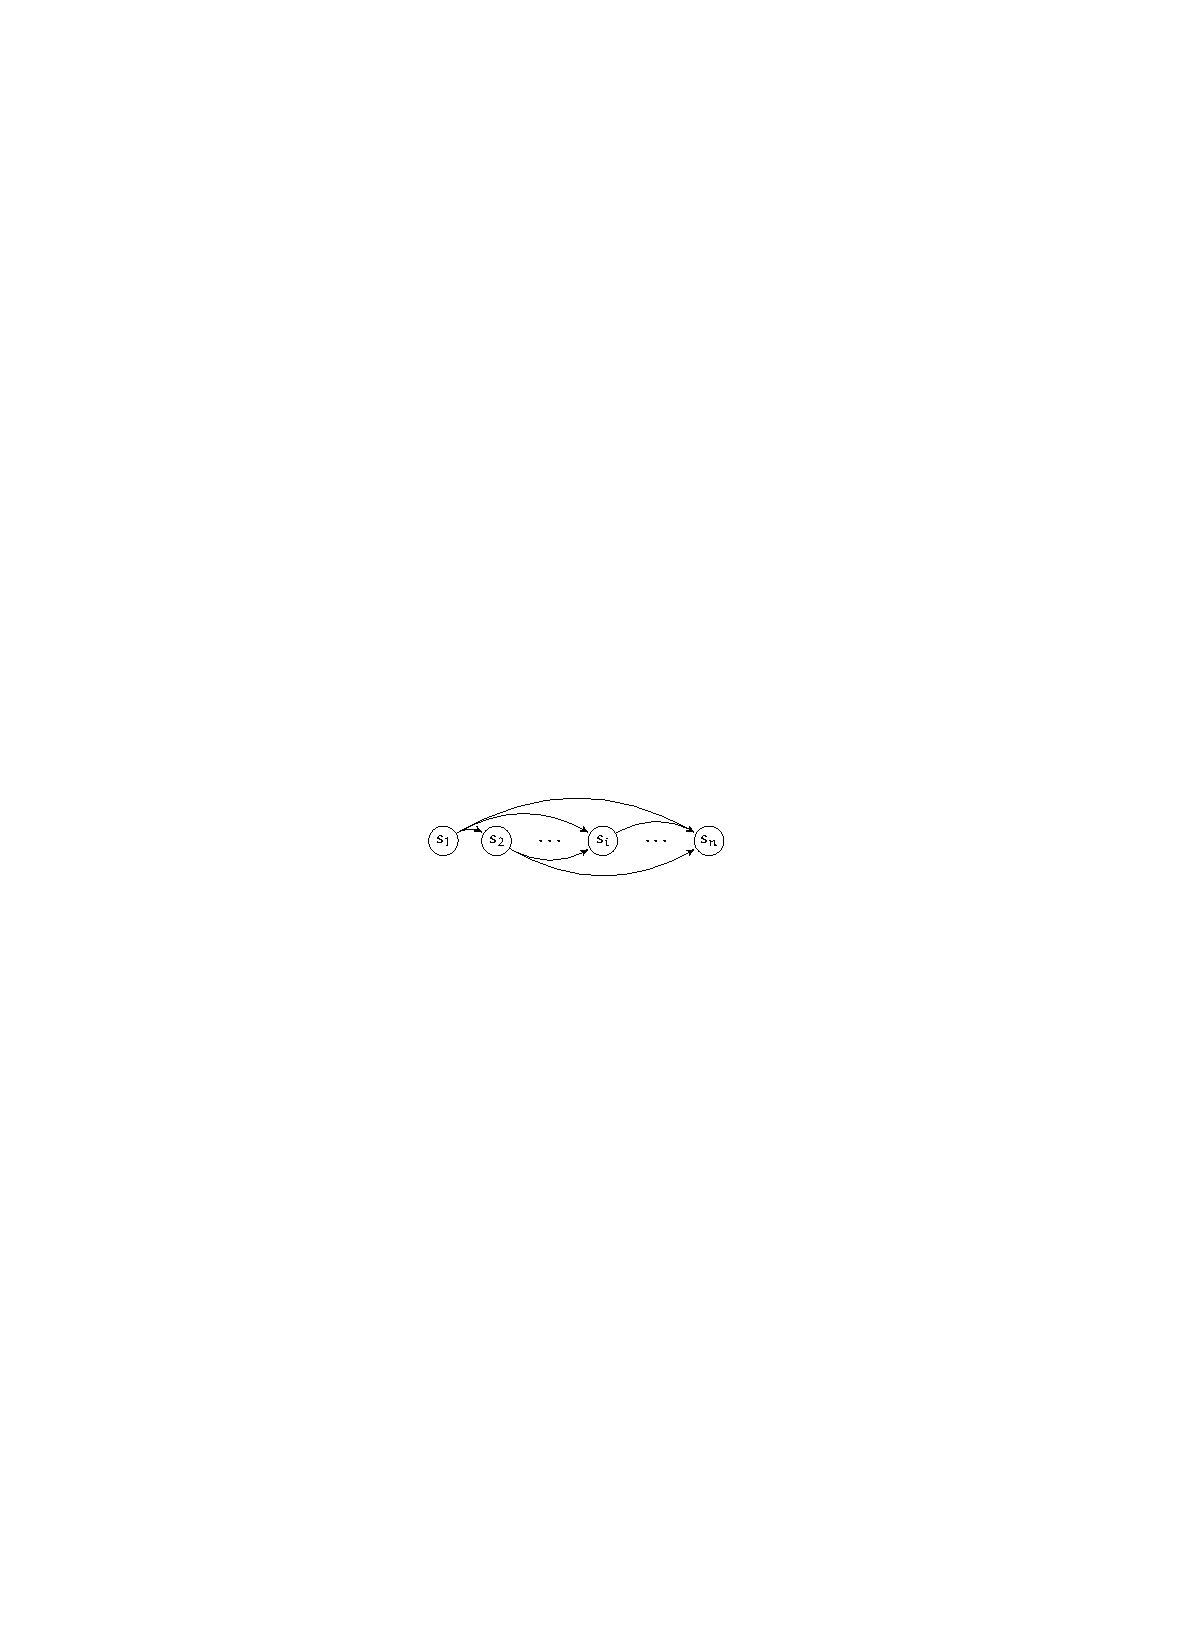
\includegraphics{./f2.pdf}
\end{center}

نمایش آن با ماتریس مجاورت (نگاه کنید به بخش ۱.۵، صفحه ۲۲) یک ماتریس مثلثاتی فوقانی است که حاوی $(1 + 2 + ... + (n - 2) + (n - 1)) = (n · (n - 1) / 2)$ بار مقدار 1 است. این نوع DAG با فرمول عبارت مطابقت دارد.

پاسخ ۳. شش مرحله از الگوریتم در شکل ۷.۱۴ نشان داده شده است. گره‌های کاندید
به رنگ خاکستری (روشن یا تیره) هستند؛ گره‌های انتخاب شده به رنگ خاکستری تیره هستند.
در گراف G، رأس‌های خاکستری کاندید برای انتقال به صف S هستند. در قسمت (ج) شکل،
رأس‌های b و f کاندید هستند. رأس b (به رنگ خاکستری تیره) به طور دلخواه انتخاب می‌شود.

نتیجه به دست آمده پس از مرحله (f) یک صف S حاوی رئوس $a، c، b، f، e، d$ است.

پاسخ ۴. در الگوریتم پس از آن، رئوس اعداد صحیح هستند. تابع پیشگیری IsDAG تضمین می کند که گراف در ورودی یک DAG باشد.

\begin{latin}
    
    \begin{algorithm}
        % \caption{}\label{your_label}
        \begin{algorithmic}
            \STATE $constants:$
            \STATE EInit ⊂ N1 and EInit = {. . .} and n = card(EInit)

            \STATE $variables:$
            \STATE E ⊂ N1 and V ∈ E × E and G = (E, V) and IsDAG(G) and
            \STATE S $\in$ FIFO(EInit)
            \STATE $begin$

            \STATE $E \leftarrow EInit; V \leftarrow {. . .};$
            \STATE $InitFifo(S);$

            \WHILE{$|S| ̸= n$}
                \STATE let s such that
                \STATE $s \in E and d - G (s) = 0$
                \STATE $begin$
                \STATE $AddFifo(S, s);$
                \STATE $E \leftarrow E - {s};$
                \STATE $G \leftarrow Induced(G, E)$
                \STATE $END$

            \ENDWHILE
            \STATE $write(S)$
            \STATE $END$

        
        \end{algorithmic}
    \end{algorithm}
        
\end{latin}

\subsubsection*{پیچیدگی}

در طول اولین گذر (به ترتیب دوم، و غیره)، در بدترین حالت n راس (به ترتیب $(n - 1)$ و غیره) برای یافتن کمترین مقدار اسکن می شوند. بنابراین کل این الگوریتم در O(n²) بازدید از رئوس یا شرایط ارزیابی شده قرار می گیرد.

پاسخ ۵.
هزینه بالای راه‌حل قبلی عمدتاً به دلیل جستجوی رأسی است که درجه ورودی آن صفر است (یعنی جستجوی کمترین). اصل راه‌حل بالقوه بهتر مبتنی بر تقویت ناوردا (invariant) با همراه کردن هر راس با درجه ورودی آن است. علاوه بر این، قرار دادن رئوس‌هایی با درجه ورودی صفر، و تنها آن رئوس‌ها، در صف ورودی F حائز اهمیت است. ساختار حاصل به شرح زیر است:

نامتغیر 
فرض کنید S یک صف اولویت‌دار (FIFO) باشد که شامل مجموعه رئوس $E_{S}$ است که بر اساس ترتیب کلی سازگار با $\prec$ مرتب شده‌اند، به گونه‌ای که هر راس v از $E$ که در $E_{S}$ نباشد $v \in (E - E_{S} )$ طبق ترتیب جزئی بزرگتر از هر راس $E_{S}$ باشد. فرض کنید F صف ورودی حاوی رئوس E باشد که در $E_{S}$ نیستند و درجه ورودی آنها برابر با صفر است. در نهایت، فرض کنید L یک ساختار باشد که شامل مجموعه تمام رئوس‌های دیگر همراه با درجه ورودی آنها و مجموعه جانشین‌های آنها است.

شرط توقف
دوباره، شرط $n = |S|$ را داریم.

پیشرفت \LTRfootnote{Progression}
یک عنصر t به طور دلخواه از صف ورودی F استخراج می شود، شناسه آن در صف خروجی S قرار می گیرد و درجه ورودی آن برای هر یک از جانشینانش w به اندازه ۱ کاهش می یابد. اگر به مقدار صفر رسید، w به صف ورودی منتقل می شود.

صف خروجی S خالی است؛ مجموعه L از هر نمایش گراف ایجاد می شود و نقاط ورودی در صف ورودی F قرار می گیرند. تمام رئوس های دیگر در L باقی می مانند.

پایان \LTRfootnote{Termination}
در هر مرحله از پیشرفت، یک راس به صف S منتقل می شود: $n - |S|$ یک عبارت خاتمه پذیر قابل قبول است.

\subsubsection*{الگوریتم}

بعد از این، هر عنصر از L از سه جزء تشکیل شده است: id معرف شناسه راس، di درجه ورودی آن و suc لیست جانشینان آن است. رویه Construct به شما امکان می دهد تا نمایشی مناسب از گراف اولیه G را در ساختار داده L بدست آورید. صف ورودی F را می توان به عنوان یک صف FIFO پیاده سازی کرد زیرا عناصر آن اولویت یکسانی دارند.


\begin{latin}
    
    \begin{algorithm}
        % \caption{}\label{your_label}
        \begin{algorithmic}
            \STATE $constants:$
            \STATE LL = {(id, di, suc) | id $\in$ E and di $\in$ N1 and suc $\subseteq$ E} and
            \STATE E ⊂ N1 and E = {. . .} and V $\in$ E $\times$ E and V = {. . .} and
            \STATE $G = (E, V)$ and IsDAG(G) and n = card(E)

            \STATE $variables:$
            \STATE S $\in$ FIFO(E) and F $\in$ FIFO(LL) and L $\subseteq$ LL and t $\in$ L
            \STATE $begin$

            \STATE $Construct(L, G); InitFifo(F);$
            \FOR{$v \in L$}
                \IF{$v.di = 0$}
                    \STATE $L \leftarrow L - {v};$
                    \STATE $AddFifo(F, v)$
                \ENDIF
            \ENDFOR
            
            \STATE $InitFifo(S);$
            \WHILE{$|S| ̸= n$}
                \STATE $t \leftarrow HeadFifo(F);$
                \STATE $RemoveFifo(F);$
                \STATE $AddFifo(S, t.id);$
                \FOR{$w \in t.suc$}
                    \STATE $w.di \leftarrow w.di - 1;$
                    \IF{$w.di = 0$}
                        \STATE $t.suc \leftarrow t.suc - {w};$
                        \STATE $AddFifo(F, w)$
                    \ENDIF
                \ENDFOR
            \ENDWHILE
            \STATE $write(F)$
            \STATE $END$
        \end{algorithmic}
    \end{algorithm}
        
\end{latin}

آخرین اصلاح مبتنی بر اشاره گرها و ساختارهای پویا نمایش زیر را برای اسکما (ب) پاسخ به سوال ۳ ارائه می دهد:

\begin{center}
    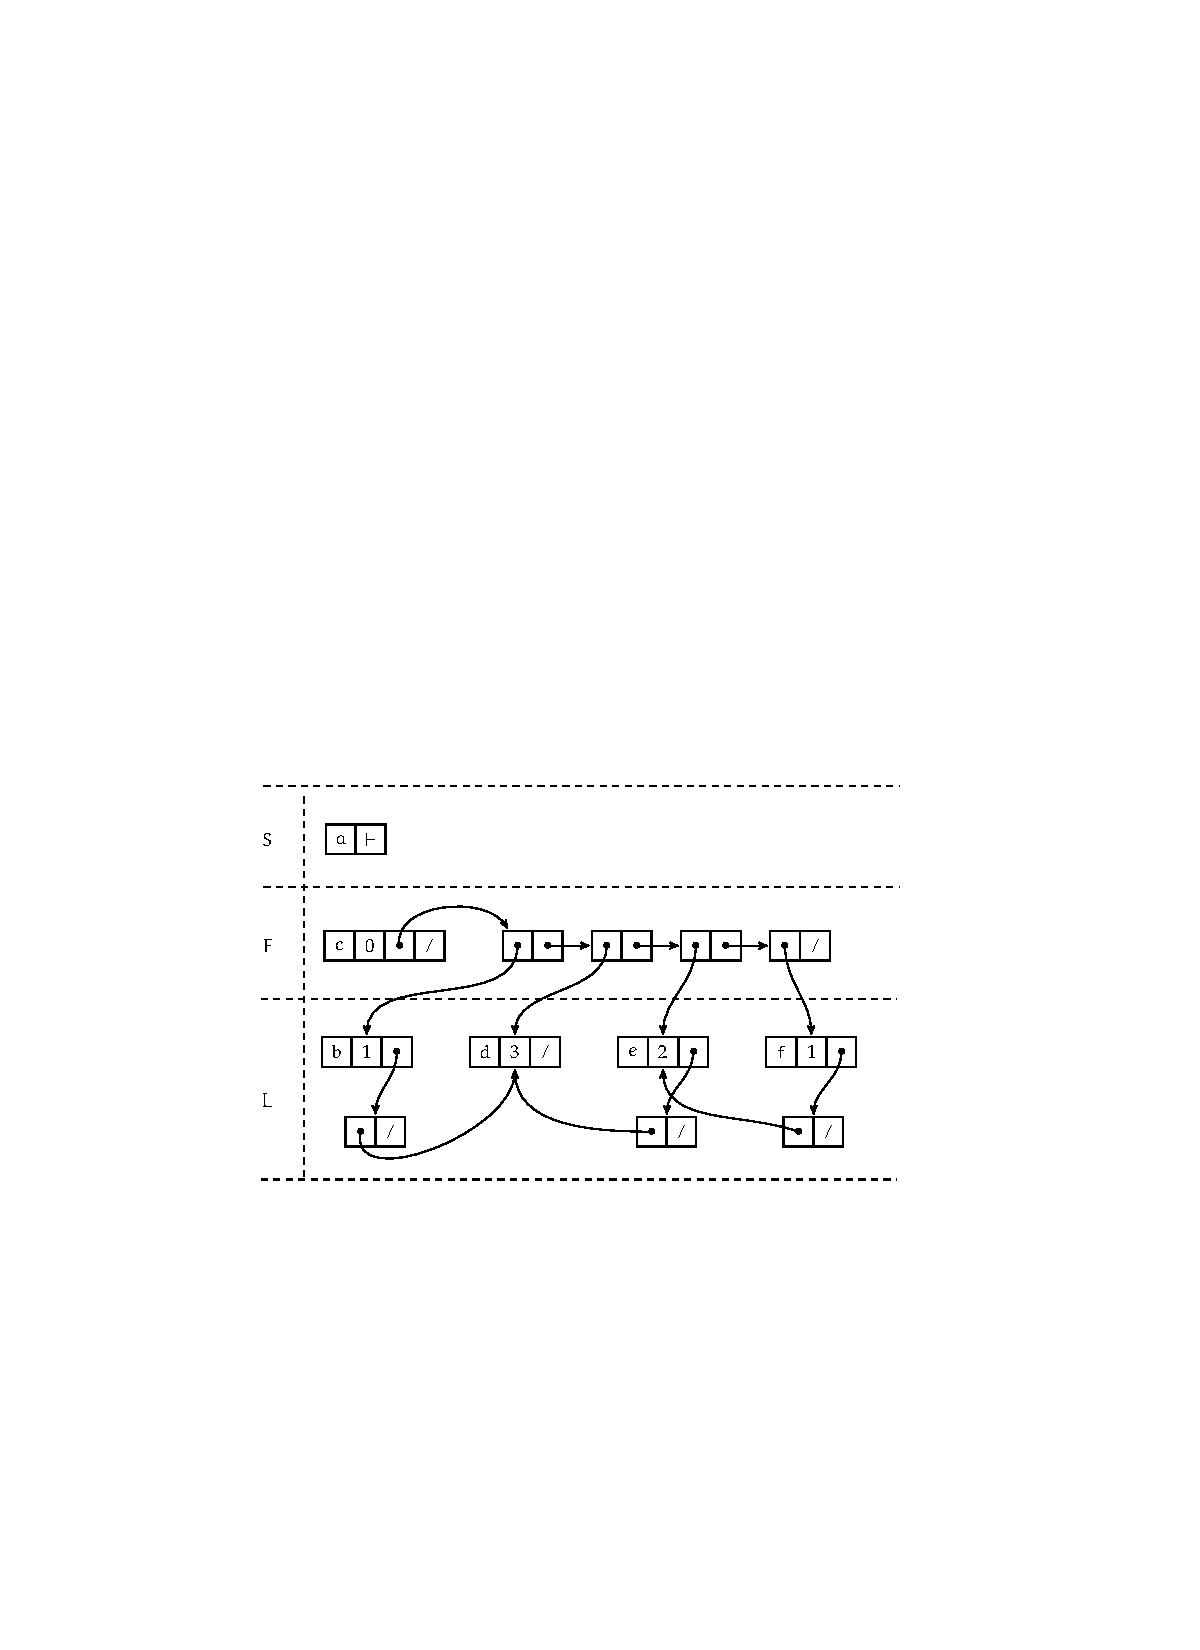
\includegraphics{./f3.pdf}

    % \imgcaption{}
\end{center}

\subsubsection*{پیچیدگی}

قابل فرض است که رویه Construct در $\theta (n + card(V))$ باشد. این در صورتی اتفاق می افتد که نمایش اولیه بر اساس لیست جانشینان باشد (نگاه کنید به شکل ۱.۳، صفحه ۲۳). تحت این شرایط، به نظر می رسد که برای بقیه الگوریتم، هر راس و هر یال یک بار در نظر گرفته شوند و عملیات روی صف ها در $\theta (1)$ باشند. در نتیجه، پیچیدگی این راه‌حل در $\theta (n + card(V))$ است. در بدترین حالت، این راه‌حل از نظر مجانبی بهتر از راه‌حل قبلی نیست، زیرا همانطور که در سوال ۲ ذکر شد، یک DAG می‌تواند به ترتیب $n^2$ یال داشته باشد. از طرف دیگر، در مورد گراف‌های غیر متراکم $(card(V) ≪ n^2)$، این راه‌حل بهتر است زیرا در $O(n + card(V))$ قرار دارد.



\end{document}
